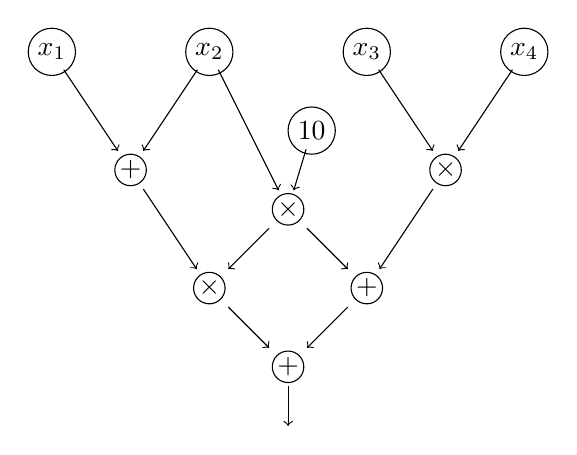
\begin{tikzpicture}
  % draw a grid starting at -4,-3 until 4,3
%  \draw[help lines] (-4,-3) grid (4, 3);

  \draw (-3, 3) circle [radius=0.3] node (x1) {$x_1$};
  \draw (-1, 3) circle [radius=0.3] node (x2) {$x_2$};
  \draw ( 1, 3) circle [radius=0.3] node (x3) {$x_3$};
  \draw ( 3, 3) circle [radius=0.3] node (x4) {$x_4$};
  \draw ( 0.3, 2) circle [radius=0.3] node (const1) {$10$};
  
  \draw ( -2, 1.5) circle [radius=0.2] node (add1) {$+$};
  \draw (  0, 1) circle [radius=0.2] node (mul1) {$\times$};
  \draw (  2, 1.5) circle [radius=0.2] node (mul2) {$\times$};

  \draw ( -1, 0) circle [radius=0.2] node (mul3) {$\times$};
  \draw (  1, 0) circle [radius=0.2] node (add2) {$+$};

  \draw (  0, -1) circle [radius=0.2] node (add3) {$+$};

  \draw[->] (x1) -- (add1);
  \draw[->] (x2) -- (add1);
  \draw[->] (x2) -- (mul1);
  \draw[->] (x3) -- (mul2);
  \draw[->] (x4) -- (mul2);
  \draw[->] (const1) -- (mul1);
  \draw[->] (add1) -- (mul3);
  \draw[->] (mul1) -- (mul3);
  \draw[->] (mul1) -- (add2);
  \draw[->] (mul2) -- (add2);
  \draw[->] (mul3) -- (add3);
  \draw[->] (add2) -- (add3);
  \draw[->] (add3) -- (0, -1.75);
\end{tikzpicture}
